\documentclass[11pt,spanish]{article}
\usepackage[utf8]{inputenc}
\usepackage{babel}
\usepackage{fullpage}
\usepackage{listingsutf8}
\usepackage{mathpazo}
\usepackage{enumitem}
\usepackage{courier}
\usepackage{xcolor}
\usepackage{textcomp}
\usepackage{amsmath}
\usepackage{amssymb}
\usepackage{tikz}
\usepackage{fancyhdr}
\usepackage{graphics}

\newcommand{\titulo}{Certamen 2, sábado 19 de noviembre de 2011}
\newcommand{\cc}[1]{\hfil\texttt{#1}\hfil}
\newcommand{\pond}[1]{[{\small\textbf{#1\%}}]}

\pagestyle{fancy}
\lhead{%
  {\Large\bfseries Programación---\titulo} \\
  Nombre: \nombre\hfill
  Rol:    \rol
  \vspace{2ex}
}
\chead{}\rhead{}\lfoot{}\cfoot{}\rfoot{}
\renewcommand{\headrulewidth}{0pt}
\addtolength{\headheight}{7ex}
\headsep=4ex


\newcommand{\onelinerule}{\rule[2.3ex]{0pt}{0pt}}
\newcommand{\twolinerule}{\rule[6.2ex]{0pt}{0pt}}
\newcommand{\respuesta}{\framebox[\textwidth]{\twolinerule}}
\newcommand{\nombre}{%
  \begin{tikzpicture}[xscale=.4,yscale=.7]
    \draw (0, 0) rectangle (22, 1);
  \end{tikzpicture}%
}
%\newcommand{\rol}   {\framebox[0.3\textwidth]{\onelinerule}}
\newcommand{\rol}{%
  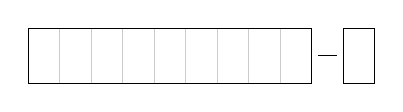
\begin{tikzpicture}[xscale=.4,yscale=.7]
    \draw[gray!40] ( 0, 0) grid      ( 9, 1);
    \draw          ( 0, 0) rectangle ( 9, 1);
    \draw          (10, 0) rectangle (11, 1);
    \draw (9 + .2, .5) -- (10 - .2, .5);
  \end{tikzpicture}%
}
\newcommand{\li}{\lstinline}
\providecommand{\pond}[1]{[{\small\textbf{#1\%}}]}

\lstdefinelanguage{py}{%
  classoffset=0,%
    morekeywords={%
      False,class,finally,is,return,None,continue,for,lambda,try,%
      True,def,from,nonlocal,while,and,del,global,not,with,print,%
      as,elif,if,or,yield,assert,else,import,pass,break,except,in,raise},%
    keywordstyle=\color{black!80}\bfseries,%
  classoffset=1,
    morekeywords={int,float,str,abs,len,raw_input,exit,range,min,max,%
      set,dict,tuple,list,bool,complex,round,sum,all,any,zip,map,filter,%
      sorted,reversed,dir,file,frozenset,open,%
      array,zeros,ones,arange,linspace,eye,diag,dot},
    keywordstyle=\color{black!50}\bfseries,%
  classoffset=0,%
  sensitive=true,%
  morecomment=[l]\#,%
  morestring=[b]',%
  morestring=[b]",%
  stringstyle=\em,%
}

\lstdefinelanguage{testcase}{%
  moredelim=[is][\bfseries]{`}{`},%
  backgroundcolor=\color{gray!20},%
}

\lstdefinelanguage{file}{%
  frame=single,%
}

\lstset{language=py}
\lstset{basicstyle=\ttfamily}
\lstset{columns=fixed}
\lstset{upquote=true}
\lstset{showstringspaces=false}
\lstset{rangeprefix=\#\ }
\lstset{includerangemarker=false}

\newlist{certamen}{enumerate}{1}
\setlist[certamen]{%
  label=\arabic*.,
  font=\LARGE\bfseries,%
  labelindent=-.5in,%
  leftmargin=0pt,%
  labelsep=1em%
}


\lstset{inputencoding=utf8/latin1}

\begin{document}

  \begin{enumerate}[font=\Large\bfseries]

    \item
      \pond{25}
      Indique qué es lo que imprimen los siguientes programas.

      \foreach \x in {1,2,...,8} {
        \noindent
        \begin{minipage}[b]{19.8em}
          \edef\dolisting{\noexpand\lstinputlisting[linerange=P\x-FIN\ P\x]{programas.py}}
          \dolisting
          \framebox[18em]{\rule[6ex]{0pt}{0pt}}
          \vspace{0.7em}
        \end{minipage}
      }

    \newpage
    \item
      \pond{25}
      Escriba las funciones necesarias para que el siguiente programa funcione.
      \lstinputlisting[linerange=PROGRAMA-FIN\ PROGRAMA, basicstyle=\small\ttfamily, frame=single]{libros.py}

    \newpage
    \item
      \pond{25}
      La ciudad de Pitonia tiene una alta congestión de vehículos
      circulando por sus calles.
      Las autoridades han decidido aplicar restricción vehicular
      para descongestionar la ciudad en base a las patentes de los vehículos.

      La patente de un vehículo es un string de cuatro letras y dos dígitos,
      y la restricción depende sólo del \emph{penúltimo} dígito.
      Por ejemplo, para la patente \li!GEEA78!,
      el dígito \li!7! es el utilizado para evaluar la restricción.

      La restricción vehícular de los días hábiles de la semana
      se encuentra ingresada en el diccionario \li!digitos!,
      cuyas llaves son los días de la semanas,
      y cuyos valores son tuplas de cuatro enteros que representan
      los dígitos con restricción de ese día.
      \begin{enumerate}
        \item Implemente la función \li!esta_con_restriccion(digitos, dia, patente)!,
          que indique si el vehículo está o no con restricción.
        \item Implemente la función \li!dias_con_restriccion(digitos, patente)!,
          que retorne la lista de los días en que el vehículo no puede circular.
        \item Implemente la función \li!dias_sin_restriccion(digitos, patente)!,
          que retorne el conjunto de los días en que el vehículo sí puede circular.
      \end{enumerate}
      \lstinputlisting[linerange=CASO-FIN\ CASO]{restriccion.py}

    \newpage
    \item
      \pond{25}
      La empresa de telecomunicaciones Python Está Aquí
      desea implementar un programa
      para monitorear y controlar la asignación de antenas
      para los teléfonos móviles de sus clientes
      en una zona específica de la ciudad.
      Para ello se considera la siguiente representación:
      \begin{itemize}
        \item la posición de cada antena es una tupla \li!(a, (x, y))!,
          donde \li!a! es el nombre de la antena
          y \li!(x, y)! es su ubicación en la zona, dada en kilómetros;
        \item la posición de casa cliente es una tupla \li!(c, (x, y))!,
          donde \li!c! es un identificador del cliente
          y \li!(x, y)! su ubicación en la ciudad, dada en kilómetros.
      \end{itemize}
      El máximo radio de cobertura de una antena es de 3 kilómetros.

      Implemente la función \li!mejor_antena(antenas, clientes, c)!,
      cuyos parámetros son las listas de antenas y clientes,
      junto con el identificador \li!c!
      de un cliente en particular.
      La función debe retornar el nombre de la antena
      que entrega la mejor cobertura (la más cercana) al cliente.
      Si existe más de una, elija cualquiera.
      Si no hay antenas dentro del radio de cobertura,
      debe retornar \li!None!.

      \lstinputlisting[linerange=CASO-FIN\ CASO]{antenas.py}

  \end{enumerate}
\end{document}

